%!TEX root = project.tex

\chapter{System Evaluation}
As many pages as needed.
\begin{itemize}
\item Prove that your software is robust. How? Testing etc. 
\item Use performance benchmarks (space and time) if algorithmic.
\item Measure the outcomes / outputs of your system / software against the objectives from the Introduction.
\item Highlight any limitations or opportunities in your approach or technologies used.

\section{Notebook – Applications and Results}
\subsection{Keras-NN}
We used the notebooks to handle the machine learning side of things when it came to training the agents. 
With this we had to research which libraries we would need in order to develop a neural network. After a lot of research, we decided on using the Keras, NumPy and Matplotlib open source libraries as these libraries best suited our objective. 

With this decided, one of our team members developed a notebook which showed a Neural Network in action. For this example, we used the IMDB data set as it was already built into the Keras library. This data set contains around 25,000 movie reviews from the website IMBD, each labelled with a positive and negative review. Each review has been pre-processed and encoded as a sequence of word indexes. With this set we extract some samples, training data to test against the data set and training targets to achieve with that data. 

In our example We’ve extracted 10,000 words from both the start and the end of the data set and assigned each to a testing and training variable respectively. With this set up, the model can be set up accordingly. We’ve set the model to Sequential as we wanted a linear stack of layers for this example. Once defined we can add our input, hidden and output layers to the model. The input layer is the layer where we pass in the input from the data set (The data we want to be tested). The hidden layer is used to transform the inputs received from the previous layer into a suitable value that the output layer can use. In turn, the output layer transforms the hidden layers activation's into whatever scale we wanted our output to be on. 

With the model made we then compile and fit the model to whatever specifications necessary. Once we fit and compiled these results, we then had to set the data we want to use to train the model, the number of episodes per each training session (epochs), the batch size of how many values we wanted to test against the model and the validation data, which contained the desired output and what the training data will be tested against.
\begin{figure}[H]
    \centering
    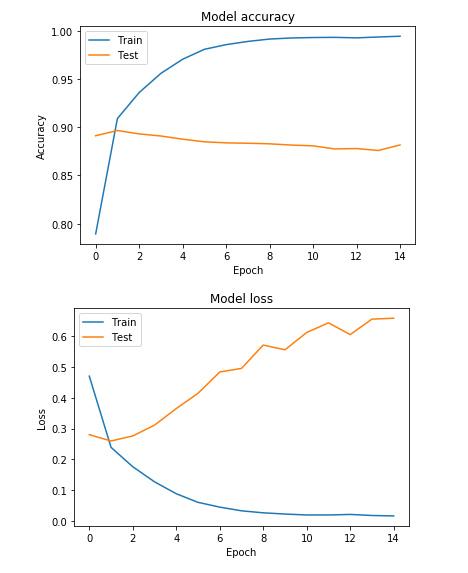
\includegraphics[width=80mm, height=80mm]{img/IMBD_results.PNG}
    \caption{Graph of the Accuracy and Loss Percentage}
    \label{fig:graph-results}
\end{figure}
The results shown in \ref{fig:graph-results} indicate that the training set got more accurate as the number of episodes increased and eventually even surpassed the set it was trained against, thus showing the robustness and efficiency of the neural network.

\subsection{10-Episode-Random}
This notebooks results are based off of random inputs sent from the notebook to the Unity environment, and the rewards from that episode were then sent back to the notebook to be processed into positive or negative values. Positive values indicated that the agent was making the correct decisions, and the negative values indicated that the agent was making the wrong choices. 

Due to the fact that the inputs to the agent were random, if the agent were to get more positive values in one episode they would not translate to the next episode, hence why the values in the graph in fig \ref{fig:10EpResults} look this way in comparison to the IMDB Neural Network results in fig \ref{fig:graph-results}.

\begin{figure}[H]
    \centering
    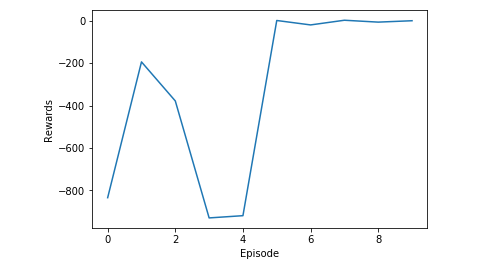
\includegraphics[width=120mm, height=50mm]{img/random10results.PNG}
    \caption{Graph of rewards from the Agent - 10 Episode Random}
    \label{fig:10EpResults}
\end{figure}

\subsection{100-Episode-Random}
For this notebook, we ran the same scene with the same scenario as the previous notebook “10-Episode-Random”. The difference between this notebook and the last is that we ran the simulation with 100 episodes in comparison to the 10 in the previous notebook. Doing this meant our simulation ran for much longer, thus giving us more data to process. Again, this is due to random inputs from the notebook, therefore the results are skewed as seen in fig \ref{fig:100EpResults}

\begin{figure}[H]
    \centering
    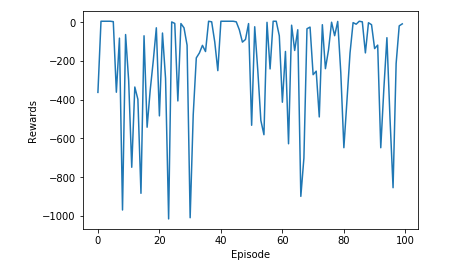
\includegraphics[width=120mm, height=50mm]{img/Large100Episode.PNG}
    \caption{Graph of rewards from the Agent - 100 Episode Random}
    \label{fig:100EpResults}
\end{figure}

\subsection{10-Episode-Large-Soccer}
With this notebook we used a different scene to the previous two notebooks mentioned. This scene was much bigger and contained more agents within the scene. This scene represents what we intended to achieve with our project, in comparison to the previous scenes with the random input. 

In this scene we’ve attached an extra C\# script called “AimForGoal” This script contains logic that distinguishes which team the agent is on. Then script then deciphers whether the agent is a goalie, a defender or an attacker, and depending on the balls position on the pitch, the agent in the best position to move towards the ball. Each agent adjusts it position at the ball to aim towards the oppositions goal. Considering we could implement the Neural Network correctly into the agents, we wanted to showcase a more accurate representation of what it would look like if we had achieved this. 

With the increase of agents and sizes, it also took a toll on the hardware of our machines when running this script. Due to this the episodes are longer, and the results accumulate slower, thus resulting in more drastic outputs. If we compare the results in fig \ref{fig:10EpLarge} with the results from the 10-Episode-Random file in fig \ref{fig:10EpResults} we can see that the first set of results had slightly more consistency when it came to the end of the episode cycle, whereas the results from this set show that the rewards outputted has a drastic change in values for each episode that ran. 

\begin{figure}[H]
    \centering
    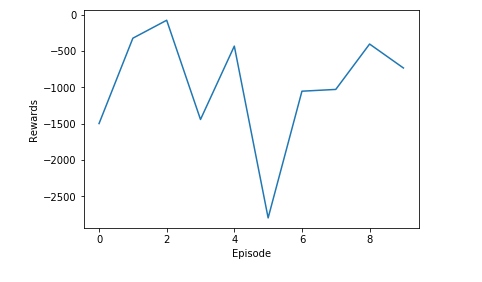
\includegraphics[width=120mm, height=50mm]{img/Large10Episode.PNG}
    \caption{Graph of rewards from the Agent - Large 10 Episode Random}
    \label{fig:10EpLarge}
\end{figure}

\subsection{100-Episode-Large-Soccer}
Similarly to the other 100 episode notebook, this is another notebook based on the previous example only running 100 episodes rather than 10. Again, with such a large scene and many agents in that scene, the simulation runs slower than all previous other examples. With the increase to the episode amount, also meant that we retrieved more data from the results. This data as seen here in fig \ref{fig:100EpLarge} is more comparable to the 100-Episode-Random results in fig \ref{fig:100EpResults}. We can see that the rewards took more of a dip during some episodes, possibly due to the fact that it ran much slower, thus adding or in this case subtracting more throughout the episode.


\begin{figure}[H]
    \centering
    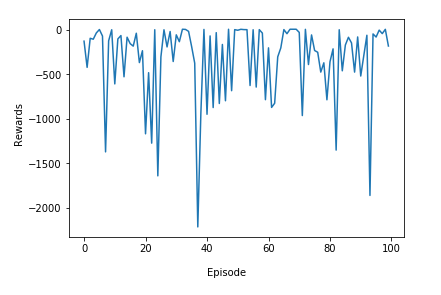
\includegraphics[width=120mm, height=50mm]{img/random100results.PNG}
    \caption{Graph of rewards from the Agent - Large 100 Episode Random}
    \label{fig:100EpLarge}
\end{figure}

\end{itemize}